%\documentclass[CJK]{beamer}
%\usetheme[left,width=5em]{Goettingen}
\usepackage{fontspec}
\usepackage{xeCJK}
\makeatletter
\newcommand{\newinfo}[1]{}
\makeatother

\usepackage{fontspec,xunicode,xltxtra,listings}
\usepackage{wasysym}
\usepackage[caption=false,font=footnotesize]{subfig}
\usepackage{url}
\usepackage{tikz}
\usepackage{tikz-uml}
\usepackage{colortbl}
\usetikzlibrary{shapes,arrows,shadows,mindmap,backgrounds,shapes.multipart}
\DeclareGraphicsExtensions{.pdf,.png,.jpg}
\graphicspath{ {./images/} }


\setbeamercovered{transparent}
\setbeamertemplate{items}[circle]

\renewcommand{\figurename}{Figure}


\newtheorem{definationfc}{Define}

\usepackage[overlap,latin]{ruby}
\renewcommand{\rubysize}{0.5}
\renewcommand{\rubysep}{-0.2ex}
\usepackage{multicol}
%\usepackage[sort&compress]{natbib}
%\usepackage{chapterbib}
\usepackage[style=authortitle]{biblatex}
\addbibresource{semver.bib}
\usepackage{multirow,tabularx}

\newcommand{\backupbegin}{
   \newcounter{framenumberappendix}
   \setcounter{framenumberappendix}{\value{framenumber}}
}
\newcommand{\backupend}{
   \addtocounter{framenumberappendix}{-\value{framenumber}}
   \addtocounter{framenumber}{\value{framenumberappendix}}
}

\newcommand{\fcshadow}[1]{%
\tikz[baseline]\path[anchor=base]
node[fill opacity=0.1] at (0.05em,-0.05em) {#1}
node[fill opacity=0.1] at (0.03em,-0.05em) {#1}
node[fill opacity=0.1] at (0.05em,-0.03em) {#1}
node[fill opacity=0.1] at (0.05em,-0.07em) {#1}
node[fill opacity=0.1] at (0.07em,-0.05em) {#1}
node at (0pt,0pt) {#1};}


\newcommand\bh{%
\tikz[remember picture, overlay]%
\coordinate(begin highlight){};%
}

\newcommand\eh{%
\tikz[remember picture, overlay]%
\coordinate (end highlight){};%
\tikz[remember picture, overlay,baseline=-0.3ex]%
\draw[yellow!50!black,line width=8pt,opacity=0.3] (begin highlight) -- (end highlight);%
}




\makeatletter
\newenvironment<>{btHighlight}[1][]
{\begin{onlyenv}#2\begingroup\tikzset{bt@Highlight@par/.style={#1}}\begin{lrbox}{\@tempboxa}}
{\end{lrbox}\bt@HL@box[bt@Highlight@par]{\@tempboxa}\endgroup\end{onlyenv}}

\newcommand<>\btHL[1][]{%
  \only#2{\begin{btHighlight}[#1]\bgroup\aftergroup\bt@HL@endenv}%
}
\def\bt@HL@endenv{%
  \end{btHighlight}%   
  \egroup
}
\newcommand{\bt@HL@box}[2][]{%
  \tikz[#1]{%
    \pgfpathrectangle{\pgfpoint{1pt}{0pt}}{\pgfpoint{\wd #2}{\ht #2}}%
    \pgfusepath{use as bounding box}%
    \node[anchor=base west, fill=orange!30,outer sep=0pt,inner xsep=1pt, inner ysep=0pt, rounded corners=3pt, minimum height=\ht\strutbox+1pt,#1]{\raisebox{1pt}{\strut}\strut\usebox{#2}};
  }%
}
\makeatother

\setCJKmainfont[BoldFont=Hiragino Kaku Gothic Pro W6]{Hiragino Kaku Gothic Pro}
\setCJKsansfont[BoldFont=Hiragino Mincho Pro W6]{Hiragino Mincho Pro}
\setCJKmonofont[BoldFont=Hiragino Kaku Gothic Pro W6]{Hiragino Kaku Gothic Pro}
%\usefonttheme{structureitalicserif}
\usefonttheme{serif}
\setmainfont{Source Sans Pro}
\setsansfont{Source Sans Pro} %[Mapping=tex-text]
\setmonofont{Source Code Pro}
% \setmonofont{Lucida Sans Typewriter}
% \setbeamerfont{frametitle}{family=\fontspec{Apple Garamond}}
% \setbeamerfont{block title}{family=\fontspec{Apple Garamond}}

\def\beamer@linkspace#1{%
  \begin{pgfpicture}{0pt}{-1.5pt}{#1}{5.5pt}
    \pgfsetfillopacity{0}
    \pgftext[x=0pt,y=-1.5pt]{.}
    \pgftext[x=#1,y=5.5pt]{.}
  \end{pgfpicture}}


\lstset{tabsize=4, %
  language=Java,
  escapechar=`,
  frame=shadowbox, commentstyle=\color{red!50!green!50!blue!50},
  rulesepcolor=\color{red!20!green!20!blue!20},
  keywordstyle=\color{blue!90}\bfseries,
  showstringspaces=false,
  stringstyle=\ttfamily,
  keepspaces=true, %
  breakindent=22pt, %
  numbers=left,%
  stepnumber=1,%
  numberstyle=\scriptsize, %
  basicstyle=\scriptsize\ttfamily, %
  showspaces=false, %
  flexiblecolumns=true, %
  breaklines=true, %
  breakautoindent=true,%
  breakindent=4em, %
  aboveskip=0.5em, %
  fontadjust,
  captionpos=t,
  framextopmargin=2pt,framexbottommargin=2pt,abovecaptionskip=-3pt,belowcaptionskip=3pt,
  xleftmargin=1.5em,xrightmargin=0.5em, %
  texcl=true,
  extendedchars=false,columns=flexible,mathescape=true,
  numbersep=0.5em,
}


%\let\oldfootnotesize\footnotesize
%\renewcommand*{\footnotesize}{\oldfootnotesize\tiny}
\AtEveryCitekey{\iffootnote{\tiny}{}}
%\appto\citesetup{\tiny}

%%% for overlay block
\tikzset{visib/.style={rectangle,text width=#1,align=flush center}}
\newenvironment{myfancyblock}%
{\begin{center}\begin{tikzpicture}}%
{\end{tikzpicture}\end{center}}%
\newcommand{\opaqueblock}[4]{
\node<#1>[#2=#3] (X) {#4};
}
%%%%%%%%%%%%%%%%%%%%%%%%%%%%%%%%%%%%%%%%%%%%%%%%%%%%%%%%%%%%%%%%%%%%%%%%


\title[SemVerと互換性をMavenで調査]{Semantic Versioning versus Breaking Changes: A Study of the Maven Repository}

\subtitle[MD輪講]{MD輪講}

\author[大阪大学大学院CS専攻 楊嘉晨]{博士後期課程3年\quad{}楊 嘉晨}
\institute[楠本研]{大阪大学大学院 \quad コンピュータサイエンス専攻 \quad 楠本研究室}
\date{2015年05月28日(木)}

\mode<article>{\providecommand{\imageheight}{0.2\textheight}}
\mode<presentation>{\providecommand{\imageheight}{0.4\textheight}}


%%%%%%%%%%%%%%%%%%%%%%%%%%%%%%%%%%%%%%%%%%%%%%%%%%%%%%%%%%%%%%%%%%%%%%%%
\begin{document}

\mode<presentation>{

\providecommand{\newblock}{\\}
\providecommand{\toprule}{\hline}
\providecommand{\midrule}{\hline}
\providecommand{\bottomrule}{\hline}
\providecommand{\itemtitle}[1]{\item \alert{#1} \quad{} }
}

\mode<article>{
\renewenvironment{columns}{\begin{multicols}{2}}{\end{multicols}\\}
\renewenvironment{column}[1]{}{}
}

\XeTeXlinebreaklocale "jp"
\XeTeXlinebreakskip = 0pt plus 1pt

\frame{\titlepage}
\mode<article>{\maketitle}

%\begin{frame}<trans|beamer>[shrink=10]{目次}
%\tableofcontents[sectionstyle=show/hide,subsectionstyle=hide,subsubsectionstyle=hide]
%\end{frame}

\AtBeginSection[]{
  \begin{frame}<trans|beamer|handout|notes>[shrink=5]
%\Huge\insertsection
\tableofcontents[sectionstyle=show/shaded,subsectionstyle=show/show/hide]
  \end{frame}
}
%%%%%%%%%%%%%%%%%%%%%%%%%%%%%%%%%%%%%%%%%%%%%%%%%%%%%%%%%%%%%%%%%%%%%%%%
\section{背景}

\subsection{著者情報と出典}
\begin{frame}{著者情報と出典}{Authors and Publication}
{\large Semantic Versioning versus Breaking Changes:
A Study of the Maven Repository
\footfullcite{raemaekers2014semantic}}
\begin{columns}
\begin{column}{0.8\textwidth}
\begin{itemize}
\item[出典] SCAM 2014, Victoria, Canada
\item[著者] Steven Raemaekers\dag, \\ \textcolor{red}{Arie van Deursen}\ddag,\\ Joost Visser\dag
{\small
\item[\dag] Software Improvement Group, Amsterdam, The Netherlands
\item[\ddag] Technical University Delft, The Netherlands
}
\end{itemize}
\end{column}
\begin{column}{0.2\textwidth}
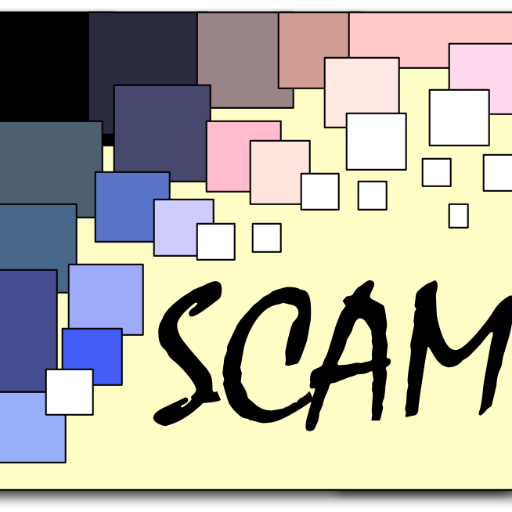
\includegraphics[width=\textwidth]{scamlogo}

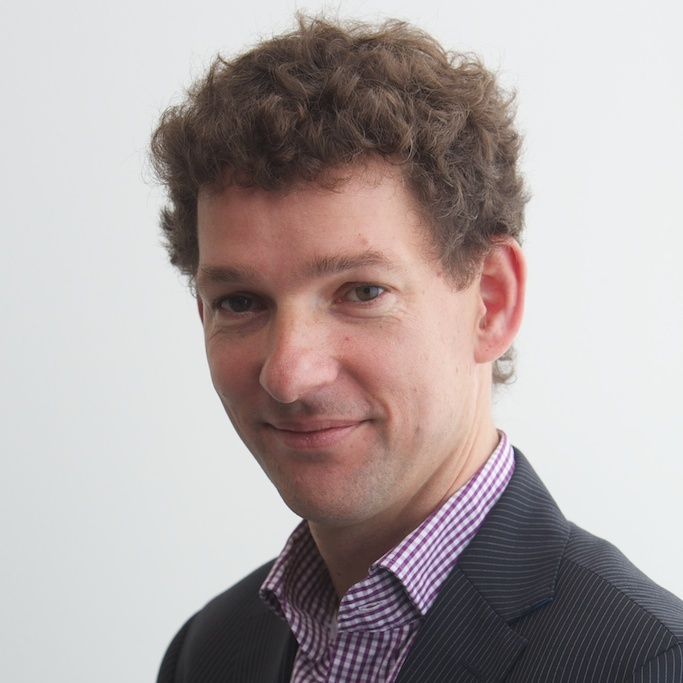
\includegraphics[width=\textwidth]{Deursen}
\end{column}
\end{columns}
\end{frame}
%%%%%%%%%%%%%%%%%%%%%%%%%%%%%%%%%%%%%%%%%%%%%%%%%%%%%%%%%%%%%%%%%%%%%%%%

%%%%%%%%%%%%%%%%%%%%%%%%%%%%%%%%%%%%%%%%%%%%%%%%%%%%%%%%%%%%%%%%%%%%%%%%
\subsection{セマンティックバージョニング}
\begin{frame}{セマンティックバージョニング}{Background: Semantic Versioning}
\vspace{-0.2em}
\begin{center}
\huge \textcolor{red}{3}.\textcolor{green!80!black}{19}.\textcolor{blue}{2} 
\end{center}
\pause

バージョンナンバーを上げるには、
\footnote{\url{http://semver.org/lang/ja/}}
\begin{itemize}
\item[\textcolor{red}{major}] APIの変更に \textcolor{red}{互換性のない} 場合
\item[\textcolor{green!80!black}{minor}] 後方互換性があり \textcolor{green!80!black}{機能性を追加した} 場合
\item[\textcolor{blue}{patch}] 後方互換性を伴う \textcolor{blue}{バグ修正} をした場合
\end{itemize}

\begin{overlayarea}{\textwidth}{0.3\textheight}
\vspace{0.2em}
\only<3,4>{
これらルールは既存のソフトウェアに広く使われてあり、全てのソフトウェアに普及すべし
\vspace{-0.2em}\pause
\begin{flushright}
\small Tom Preston-Werner 氏, Gravatars及びGitHubの共同創設者
\end{flushright}
}
\only<5->{
実際、バージョンナンバーは本当にセマンティックバージョニング(以下SemVerと略称)の原則を守っているか?}
\end{overlayarea}
\end{frame}
%%%%%%%%%%%%%%%%%%%%%%%%%%%%%%%%%%%%%%%%%%%%%%%%%%%%%%%%%%%%%%%%%%%%%%%%
\subsection{SemVerとAPIの後方互換性}
\begin{frame}{SemVerと互換性}{Semantic Versioning and API Compatibility}
ソフトウェアやライブラリーのユーザーにとって、APIの\fcshadow{後方互換性}は重要である

\begin{tikzpicture}[grow=right]
\node (sa) at (0,0) {ソフトウェアA};
\node (lb1) at (6,1) {ライブラリーB: 1.2};
\node (lb2) at (6,0) {ライブラリーB: 1.\textcolor{green!80!black}{3}};
\node (lb3) at (6,-1) {ライブラリーB: \textcolor{red}{2}.0};
\path[draw               ,thick,->]<1> (sa.east) -> (lb1.west);
\path[draw=green!80!black,thick,->]<2> (sa.east) -> (lb2.west);
\path[draw=red           ,thick,->]<3-> (sa.east) -> (lb3.west);
\end{tikzpicture}

\uncover<4>{SemVerの原則が守っていれば、安心で依存関係のライブラリーをアップグレードすることができる}
\end{frame}
%%%%%%%%%%%%%%%%%%%%%%%%%%%%%%%%%%%%%%%%%%%%%%%%%%%%%%%%%%%%%%%%%%%%%%%%
\section{Research Questions}
\subsection{調査目的と対象}
\begin{frame}{調査目的と対象}{Goal and Research Targets}
\begin{itemize}
\item[目的] バージョン番号を上げる際にAPI互換性がSemVer原則に従われているかどうか
\item[対象] Maven中央リポジトリ\footnote{\url{http://search.maven.org/
}}にあるほぼ全てのOSS
\end{itemize}
\pause
\begin{block}{Maven中央リポジトリを対象とする原因}
\begin{itemize}
\item プロジェクト間の依存関係が記述される
\item 一箇所に集まる
\item バージョン番号も明記されています
\end{itemize}
\end{block}
\end{frame}
%%%%%%%%%%%%%%%%%%%%%%%%%%%%%%%%%%%%%%%%%%%%%%%%%%%%%%%%%%%%%%%%%%%%%%%%
\subsection{調査項目}
\begin{frame}{調査項目}{Research Questions}
\begin{itemize}
\item[RQ1] 互換性に関するSemVer原則はどのぐらい従われている?
\item[RQ2] SemVer原則に従うソフトウェアは時間に亘って増えているか?
\item[RQ3] 新しいバージョンへの依存関係はどう更新されてるか?
最新版を使わぬ要因は何がある?
\item[RQ4] 廃止予定(deprecation)のタグは実際にどう使われているのか?
\end{itemize}
\pause
{\small
\begin{block}{廃止予定\texttt{@deprecated}}
API互換性を破る前に、幾つかのバージョンに予め廃止を予定したメソッド等につけるアノテーション
\end{block}
}
\end{frame}
%%%%%%%%%%%%%%%%%%%%%%%%%%%%%%%%%%%%%%%%%%%%%%%%%%%%%%%%%%%%%%%%%%%%%%%%
\section{調査手法}
\subsection{調査手法の概要}
\begin{frame}{調査手法の概要}

\begin{tikzpicture}
\node (maven) at (0,0) {
\includegraphics[width=3em]{repo}};
\node (mavent) at (0,-1) {中央リポ};
\node (jar) at (3,2) {
\includegraphics[width=3em]{jar}};
\node (jart) at (5,2) {バイナリー};
\node (metadata) at (3,0) {
\includegraphics[width=3em]{metadata}};
\node (metadatat) at (5,0) {メタ情報};
\node (java) at (3,-2) {
\includegraphics[width=3em]{java}};
\node (javat) at (5,-2) {ソース};

\node (jt) at (9,2) {互換性};

\node (m1) at (9,1) {バージョン番号};
\node (m2) at (9,0) {リリース日時};
\node (m3) at (9,-1) {依存関係};

\node (jt1) at (9,-2) {AST変更};
\node (jt2) at (9,-3) {\texttt{@Deprecated}};

\path[draw,thick,->] (maven.east) -> (jar.west);
\path[draw,thick,->] (maven.east) -> (metadata.west);
\path[draw,thick,->] (maven.east) -> (java.west);

\path[draw,thick,->] (jart.east) -> (jt.west);

\path[draw,thick,->] (metadatat.east) -> (m1.west);
\path[draw,thick,->] (metadatat.east) -> (m2.west);
\path[draw,thick,->] (metadatat.east) -> (m3.west);

\path[draw,thick,->] (javat.east) -> (jt1.west);
\path[draw,thick,->] (javat.east) -> (jt2.west);
\end{tikzpicture}

\end{frame}
%%%%%%%%%%%%%%%%%%%%%%%%%%%%%%%%%%%%%%%%%%%%%%%%%%%%%%%%%%%%%%%%%%%%%%%%
\subsection{Maven中央リポジトリ}
\begin{frame}{Maven中央リポジトリ}
2011年7月11日の時点のMaven中央リポジトリのスナップショット
\footnote{\url{http://juliusdavies.ca/2013/j.emse/bertillonage/maven.tar.gz}}
を取ってきて\footfullcite{davies2011software}、
\texttt{pom.xml}を解析し、プロジェクト間に依存関係でリンク付け\footfullcite{raemaekers2013maven}

\vspace{1em}

\begin{tabular}{l|r|r|r}
& プロジェクト数 & バイナリーjar & ソースjar \\
\hline
規模 & 22,205 & 148,253 & 101,413 \\
\end{tabular}

\vspace{1em}

平均、プロジェクト毎に6.7リリース
\end{frame}

%%%%%%%%%%%%%%%%%%%%%%%%%%%%%%%%%%%%%%%%%%%%%%%%%%%%%%%%%%%%%%%%%%%%%%%%
\subsection{APIの後方互換性を判断する基準}
\begin{frame}{APIの後方互換性を判断する基準}{Determining backward incompatible API changes
}
{\small

厳密にAPI互換性の有無を判断することは困難
  \begin{itemize}
  \item 意味的に解析や、実際にビルド・テストする必要
  \end{itemize}
\pause

代わりに本研究では\textcolor{red}{バイナリー互換性}を判断基準とする

\begin{block}{Java言語仕様にバイナリー互換性の定義
\footnote{\url{http://docs.oracle.com/javase/specs/jls/se7/html/jls-13.html
}}}
APIに変更する前後に、リンクする際にエラーが起こらないことはバイナリー互換性があること
\end{block}

\begin{block}{本研究に使った定義}
再度コンパイルし直す必要がないAPIの変更\footnote{\url{http://wiki.eclipse.org/Evolving Java-based APIs
}}
\end{block}
}

\end{frame}

%%%%%%%%%%%%%%%%%%%%%%%%%%%%%%%%%%%%%%%%%%%%%%%%%%%%%%%%%%%%%%%%%%%%%%%%
\begin{frame}{Clirr:公開APIに変更を検出ツール
\footnote{http://clirr.sourceforge.net}}{Clirr: Tool to Extract API changes}
入力:バイナリーJarファイル、出力:公開API違い

\vspace{0.5em}

\begin{tabular}{l|l}
互換性がない & 互換性がある \\
\hline
メソッドの削除 & メソッドの追加 \\
クラスの削除 & クラスの追加 \\
フィルドの削除 & フィルドの追加 \\
引数の型が変更 & 親クラスレスとに追加 \\
フィルドの型が変更 & 定数の値が変更 \\
\hline
総数:23 & 総数:20
\end{tabular}

\vspace{0.5em}

安全側に立って、検出した互換性がない修正は絶対正しいが、互換性がある変更に間違いがある
\end{frame}

%%%%%%%%%%%%%%%%%%%%%%%%%%%%%%%%%%%%%%%%%%%%%%%%%%%%%%%%%%%%%%%%%%%%%%%%
\subsection{バージョン番号の比較}
\begin{frame}{バージョン番号の比較}{Determining subsequent versions and update types}
以下の要素でライブラリーのバージョンを特定

\begin{tabular}{l|l|l}
groupId & artifactId & version \\
\hline
org.springframework & spring-core & 2.5.6 \\
\end{tabular}

\pause\vspace{0.5em}

バージョン番号の比較は Artifact API 
\footnote{\url{http://maven.apache.org/ref/3.1.1/maven-artifact}}
を使います


\pause\vspace{0.5em}

フォーマットは \texttt{MAJOR.MINOR.PATCH}、
\texttt{PATCH}がない場合に0とみなす

\pause\vspace{0.5em}

プレリリース(1.2.3-beta1や1.2.3-snapshot)は対象から外す
\end{frame}
%%%%%%%%%%%%%%%%%%%%%%%%%%%%%%%%%%%%%%%%%%%%%%%%%%%%%%%%%%%%%%%%%%%%%%%%
\subsection{ソースコードの比較と廃止パターン}
\begin{frame}{ソースコードの比較と廃止パターン}{Detecting changed functionality 
and deprecation patterns}

ソースコードはどのぐらい変更したのかをChangeDistiller\footfullcite{fluri2007change}で比較します

\begin{block}{ChangeDistiller}
入力:2つバージョンのソースコード

出力:AST上のノードの編集スクリプト
\end{block}

\pause\vspace{1em}

廃止APIはキーワード\texttt{@Deprecated}で検索し、該当するソースファイルをJDTで解析して、
廃止APIのパターンを検出します。
\end{frame}
%%%%%%%%%%%%%%%%%%%%%%%%%%%%%%%%%%%%%%%%%%%%%%%%%%%%%%%%%%%%%%%%%%%%%%%%
\section{統計的な結果}
\subsection{バージョン文字列のパターン}
\begin{frame}{バージョン文字列のパターン}
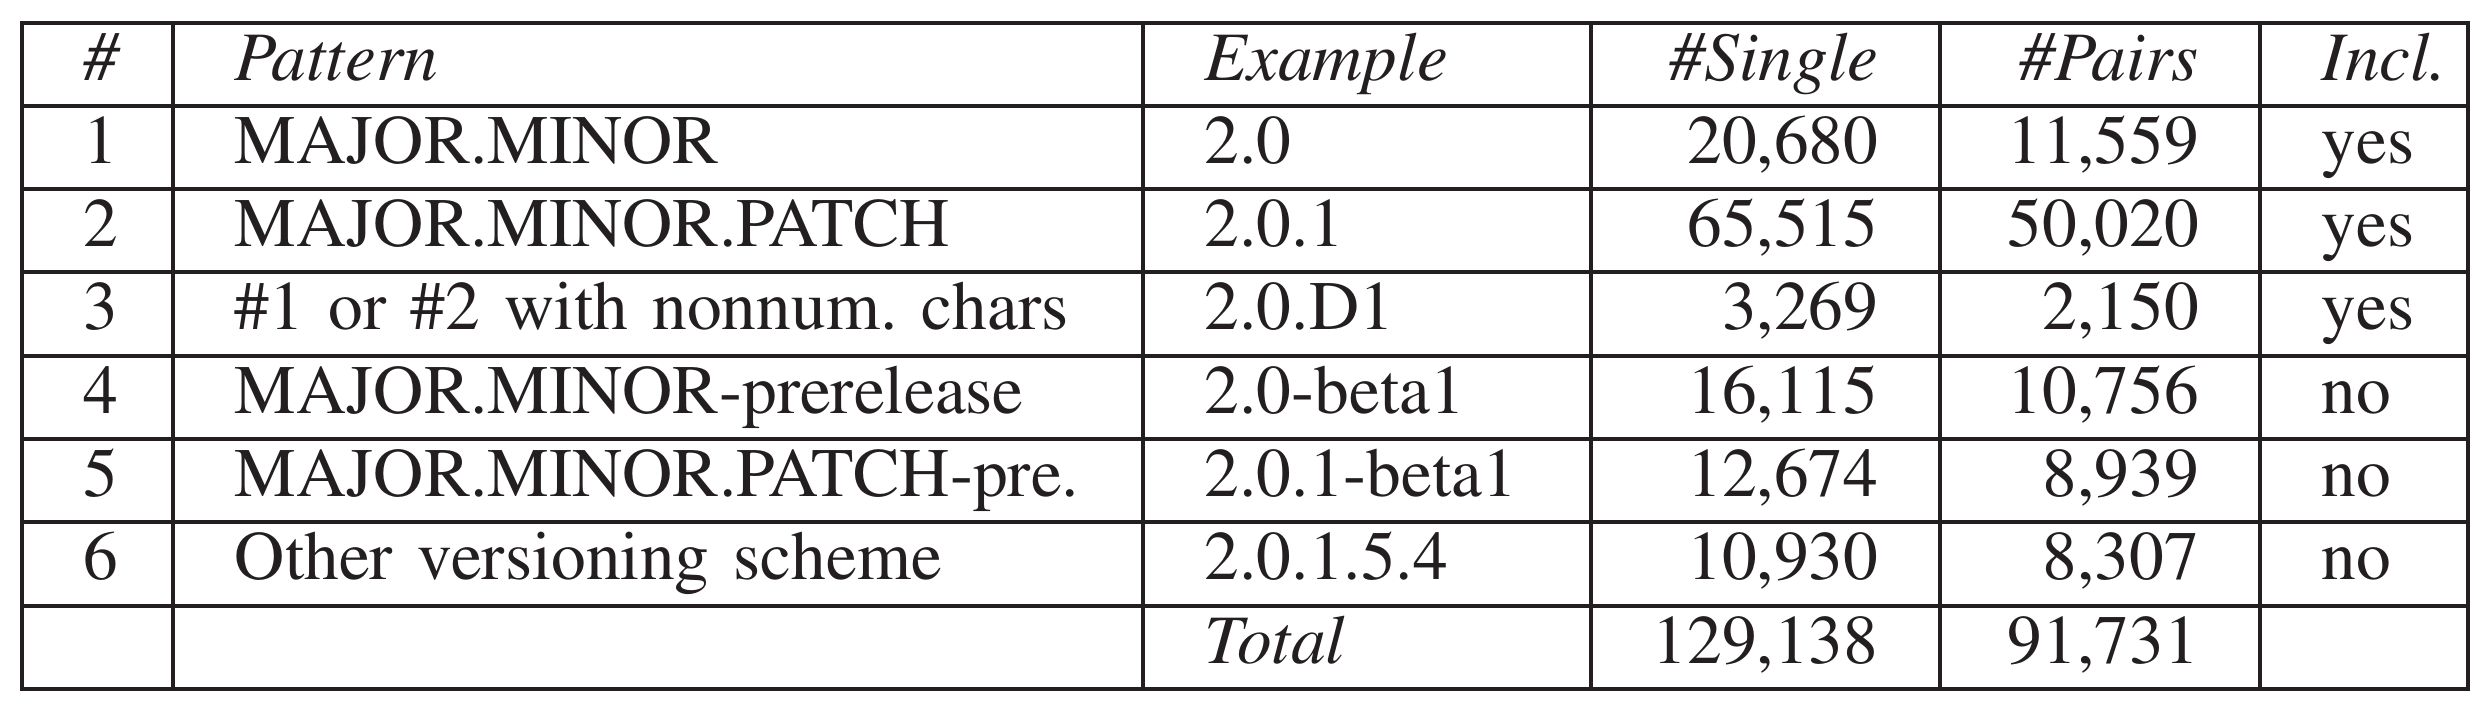
\includegraphics[width=\textwidth]{table1}

69\%のバージョン文字列はSemVerのフォーマットになっています。

22.3\%のバージョン文字列はプレリリース(4と5)である。

29\%のライブラリーは1つのリリースのみである。

\end{frame}

%%%%%%%%%%%%%%%%%%%%%%%%%%%%%%%%%%%%%%%%%%%%%%%%%%%%%%%%%%%%%%%%%%%%%%%%
\subsection{互換性が有無のAPI変更}
\begin{frame}{互換性が有無のAPI変更}

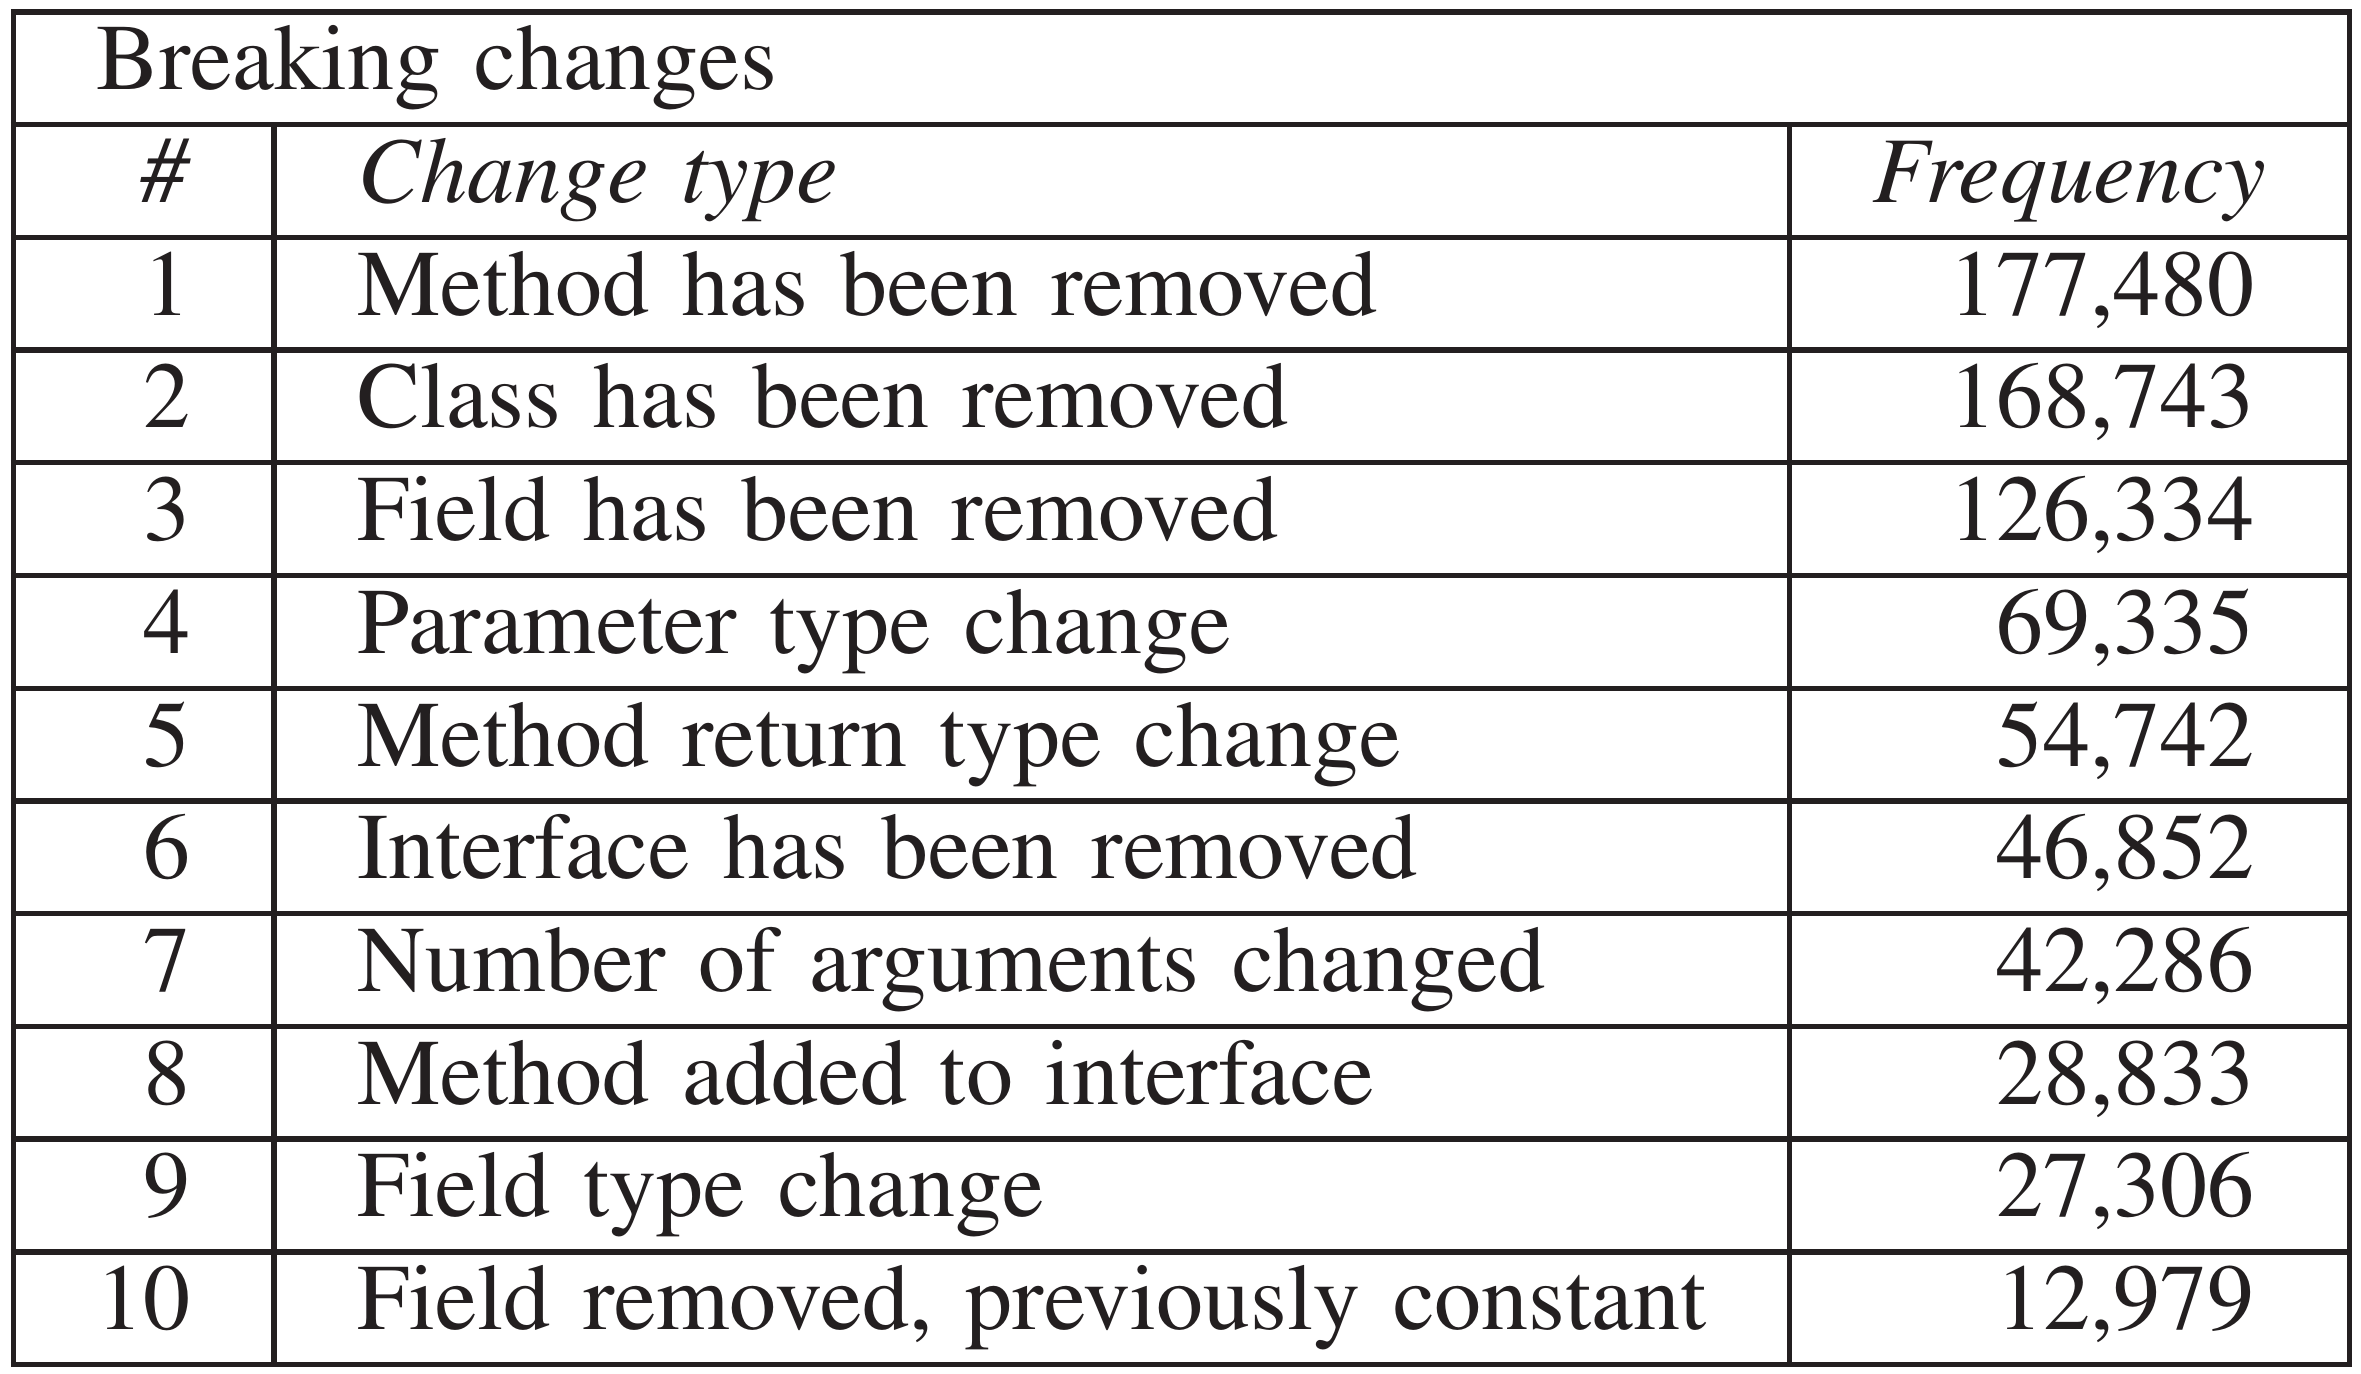
\includegraphics[width=0.48\textwidth]{table2a}
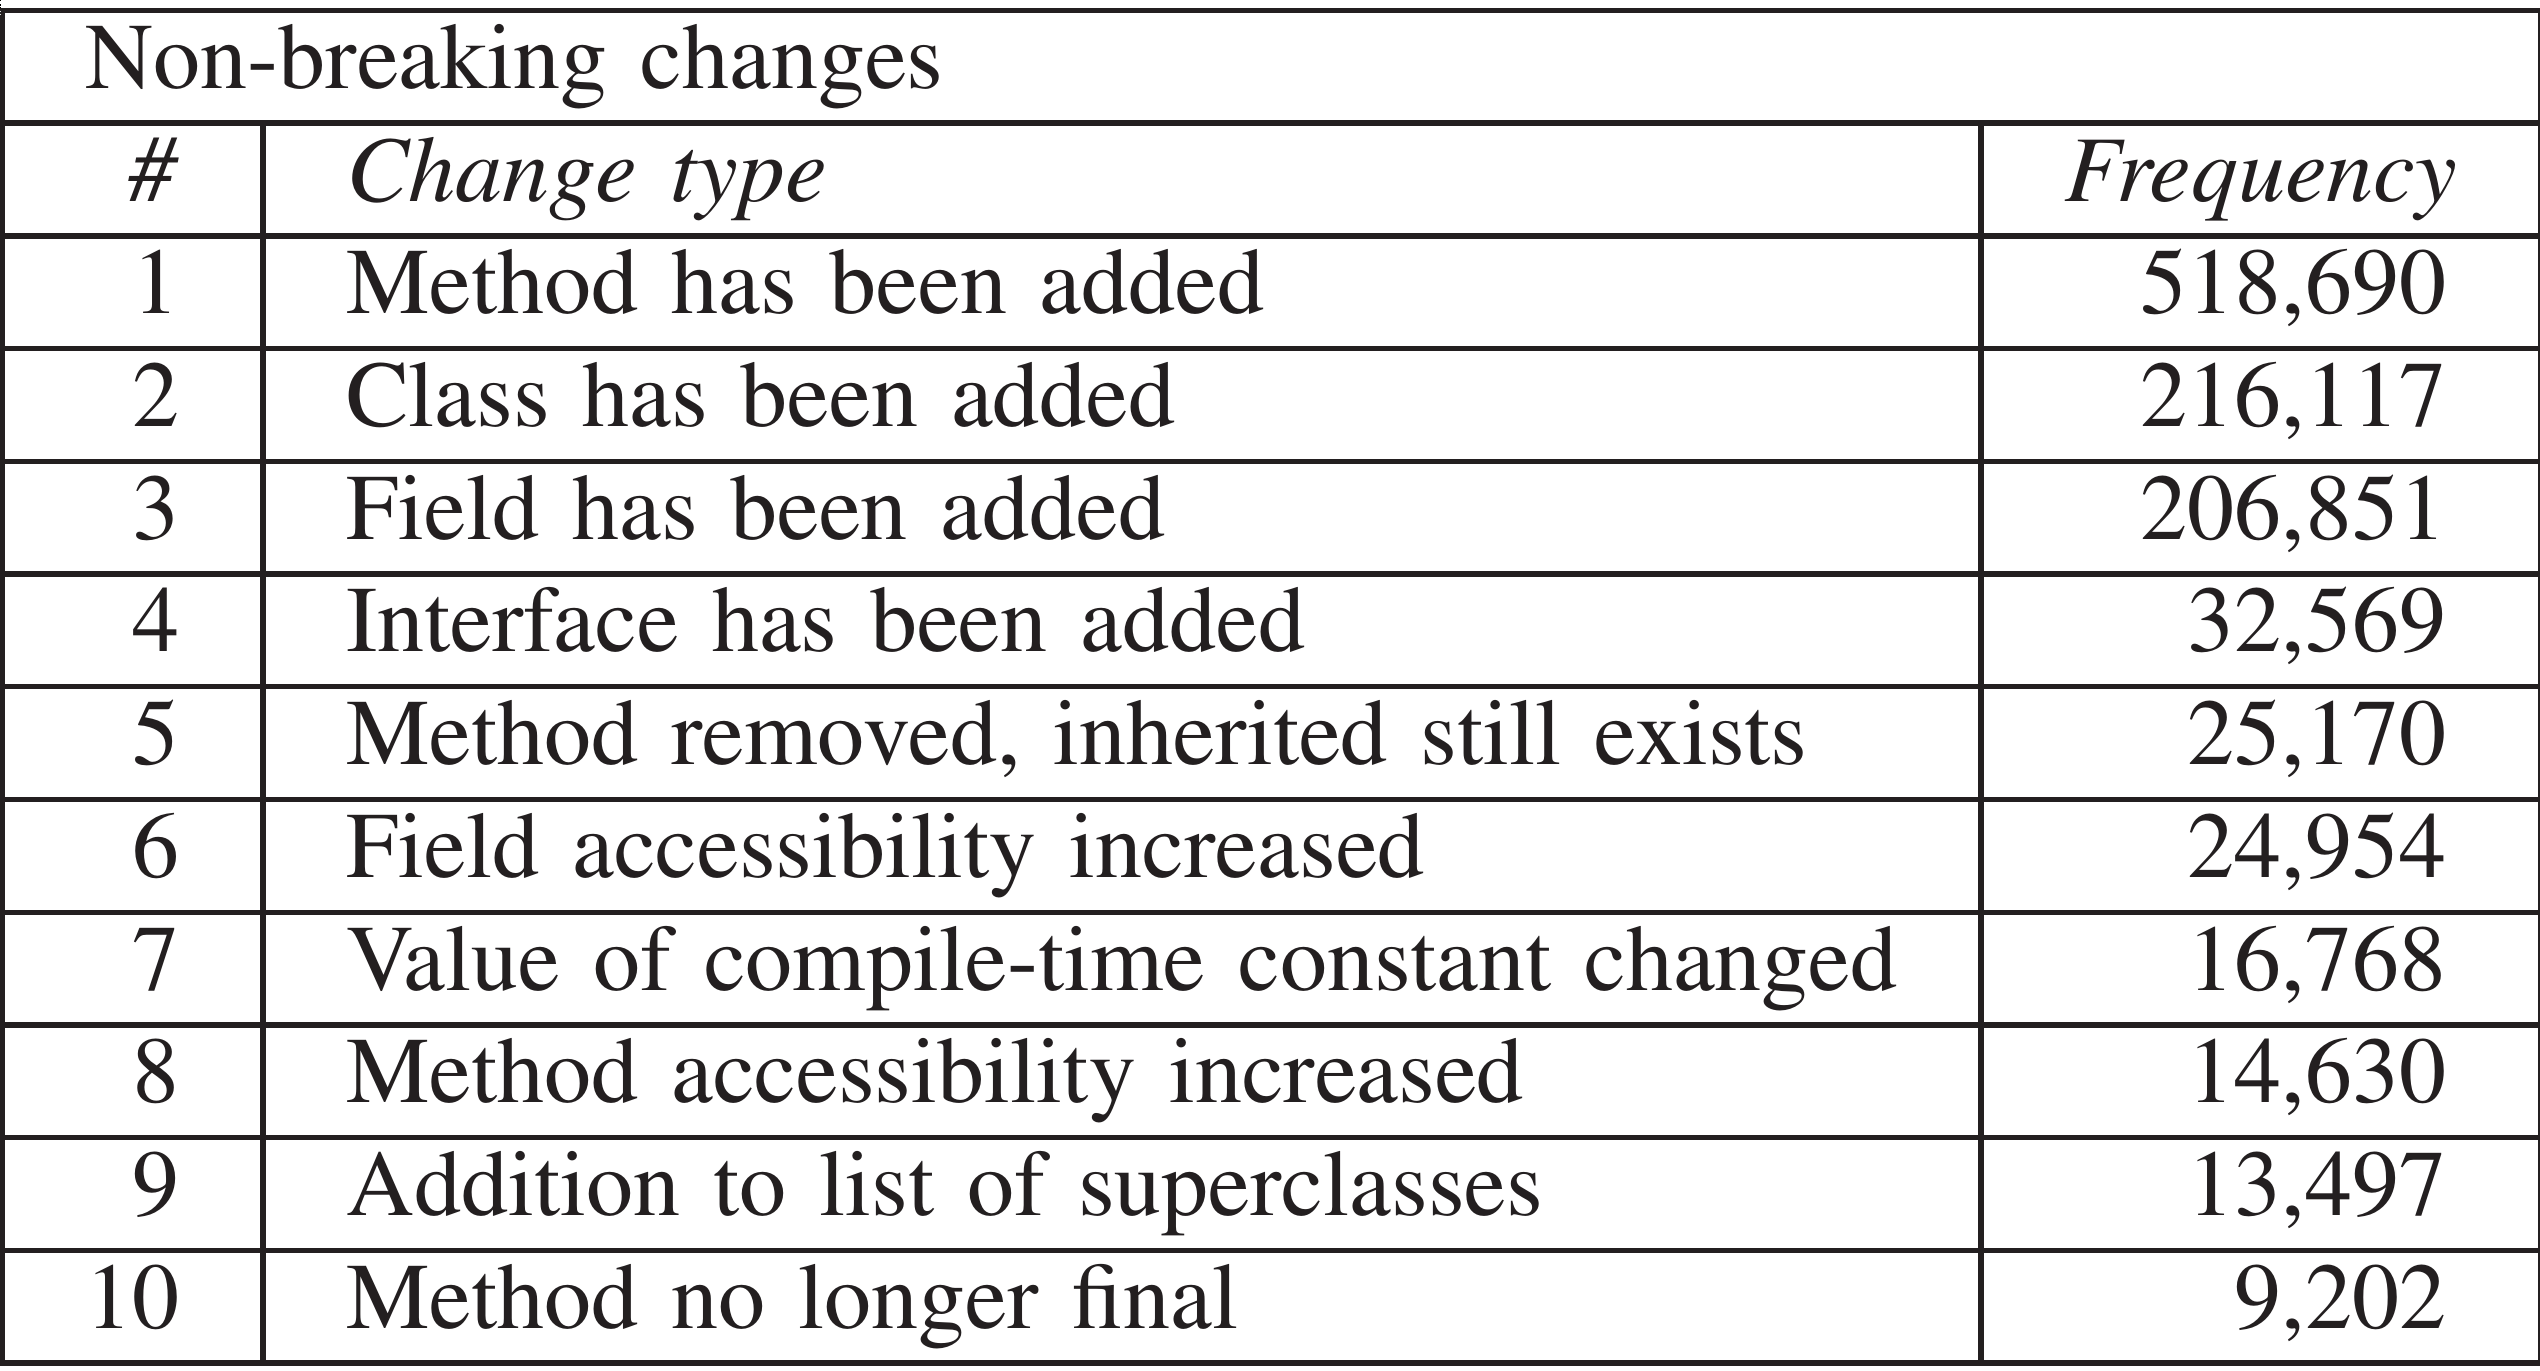
\includegraphics[width=0.51\textwidth]{table2b}

\begin{overlayarea}{\textwidth}{0.5\textheight}
\only<2->{
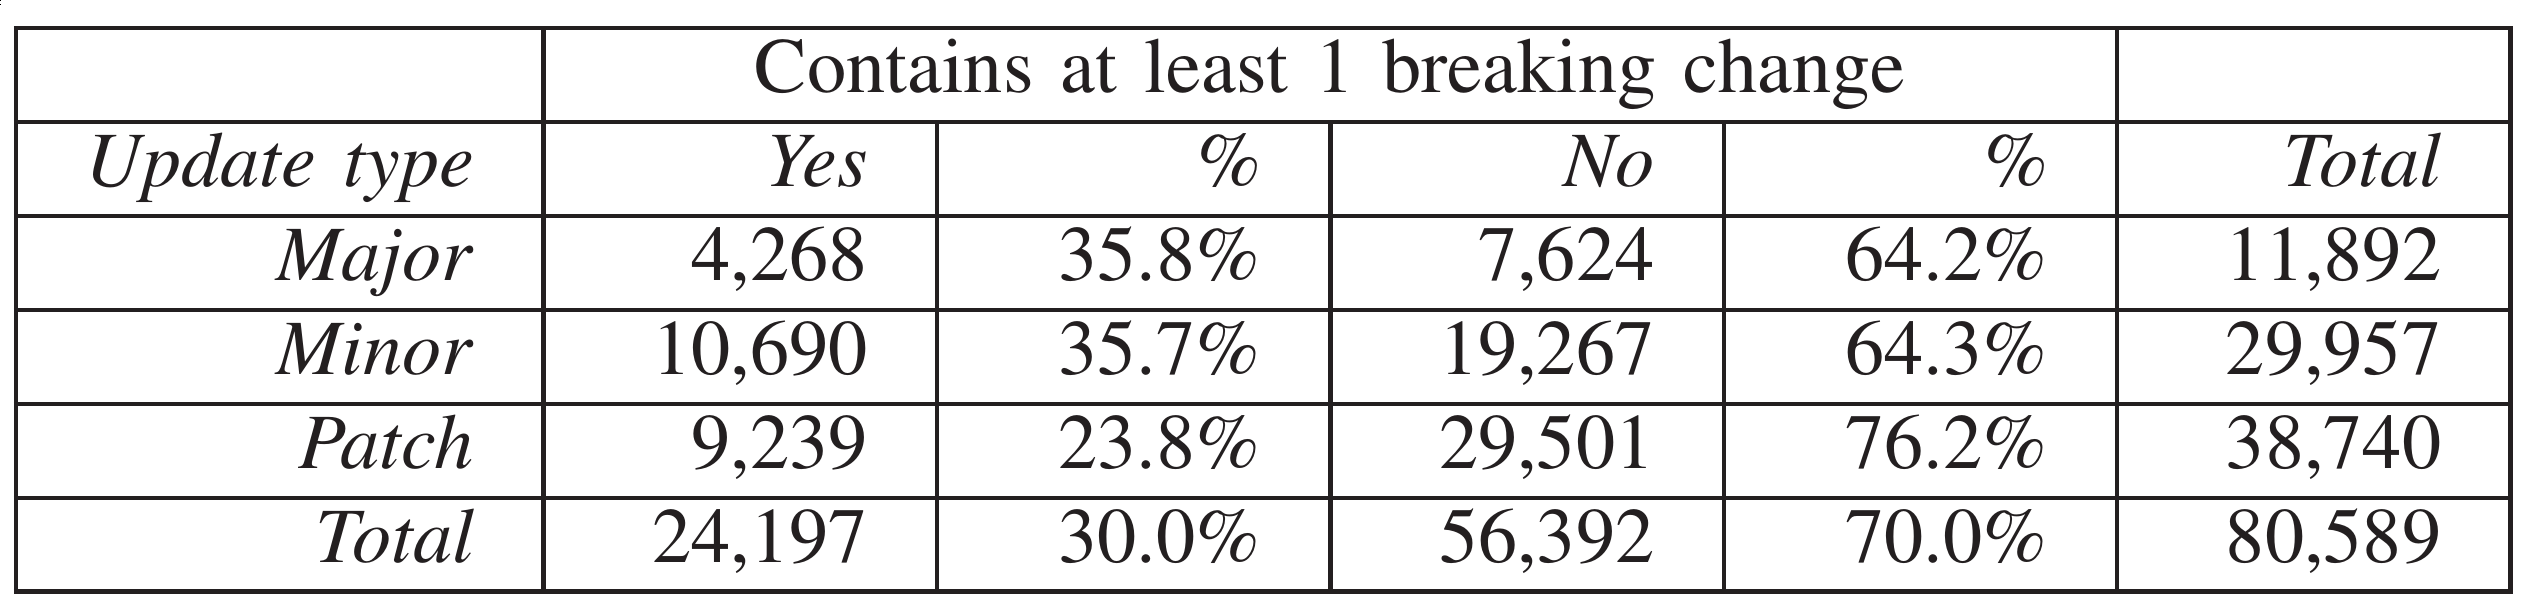
\includegraphics[width=\textwidth]{table3}

\uncover<3->{Major と Minor の使い分けは\textcolor{red}{されていない}!}
}
\end{overlayarea}
\end{frame}
%%%%%%%%%%%%%%%%%%%%%%%%%%%%%%%%%%%%%%%%%%%%%%%%%%%%%%%%%%%%%%%%%%%%%%%%
\section{調査項目の結果}
\subsection{RQ1:SemVer原則が従われているか}
\begin{frame}{RQ1:SemVer原則が従われているか}

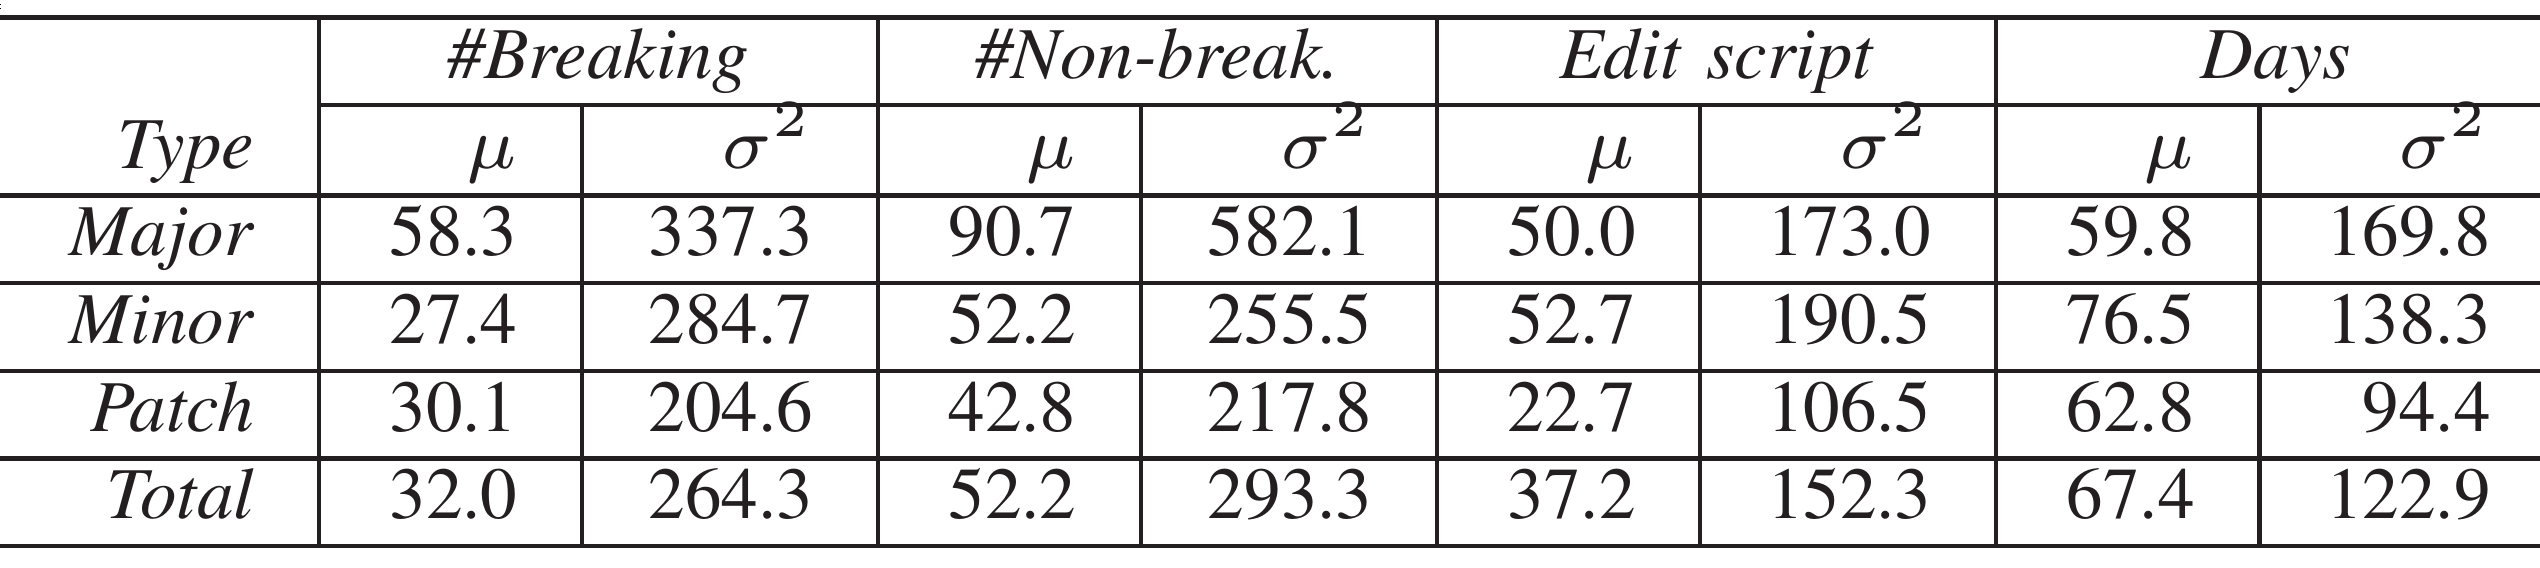
\includegraphics[width=\textwidth]{table4}

SemVer を従われていれば、Minor/Patchに互換性がない変更はないはずなのに、
実際 Minor/Patch に平均 30 ぐらいの互換性がない変更がある。

\pause\vspace{0.5em}

編集の大きさから見ると、Minor は Major より大きいが、Patchは相対的に小さい。

\pause\vspace{0.5em}

リリースの間隔から見ると、MinorはMajorより時間がかかる。
\end{frame}

%%%%%%%%%%%%%%%%%%%%%%%%%%%%%%%%%%%%%%%%%%%%%%%%%%%%%%%%%%%%%%%%%%%%%%%%
\begin{frame}{RQ1に対する回答}

{\Huge
後方互換性に関するSemVer原則は実際に\textcolor{red}{守られていない}!
}

\pause\vspace{1em}

{\Large
MinorリリースとPatchリリースには、互換性のない変更が\textcolor{red}{平均30個}ぐらいあります。
}

\end{frame}
%%%%%%%%%%%%%%%%%%%%%%%%%%%%%%%%%%%%%%%%%%%%%%%%%%%%%%%%%%%%%%%%%%%%%%%%
\subsection{RQ2:時間を亘って変わるか}
\begin{frame}{RQ2:時間を亘って変わるか}
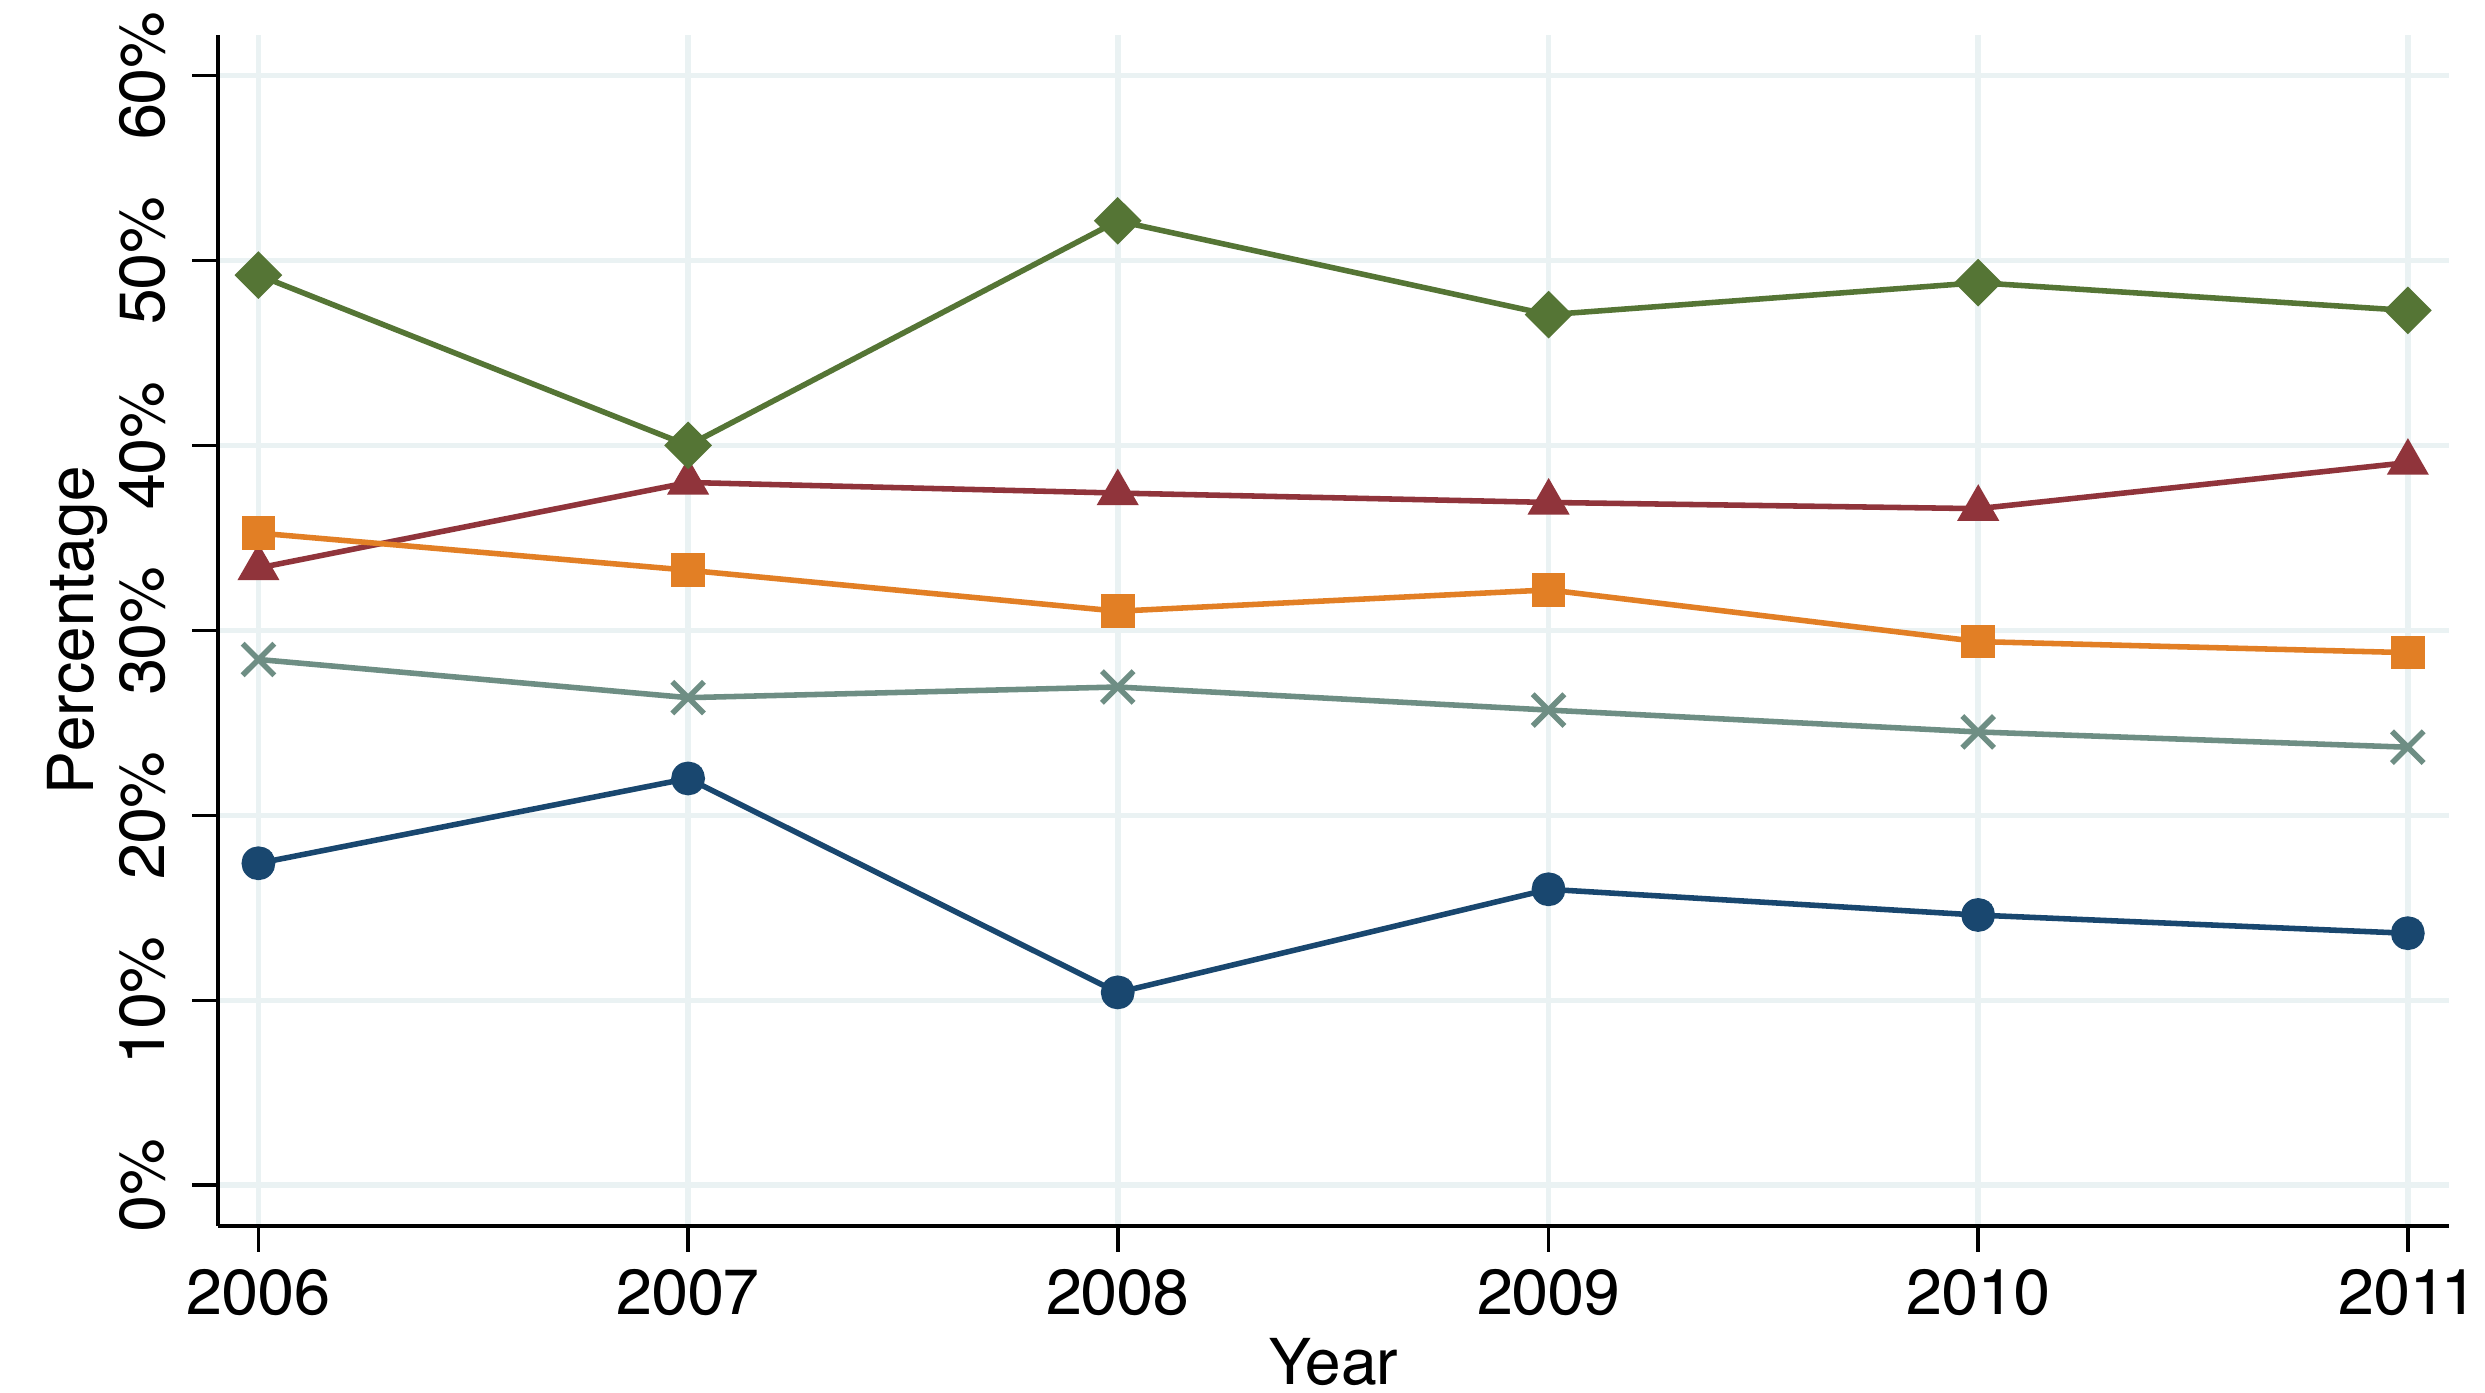
\includegraphics[width=\textwidth]{figure5a}


\includegraphics[height=1.1em]{figure5b}

\includegraphics[height=1.1em]{figure5c}

\includegraphics[height=1.1em]{figure5d}


\includegraphics[height=1.1em]{figure5e}

\includegraphics[height=1.1em]{figure5f}
\end{frame}
%%%%%%%%%%%%%%%%%%%%%%%%%%%%%%%%%%%%%%%%%%%%%%%%%%%%%%%%%%%%%%%%%%%%%%%%
\begin{frame}{RQ2に対する回答}

{\Huge
SemVer原則を守ることは近年少しぐらい\textcolor{red}{増えている}
}

\pause\vspace{1em}

{\Large
MinorとPatchリリースに互換性のない変更の割合は、
2006年の\textcolor{red}{28.4\%}から、2011年に\textcolor{red}{23.7\%}になりました。
}

\end{frame}
%%%%%%%%%%%%%%%%%%%%%%%%%%%%%%%%%%%%%%%%%%%%%%%%%%%%%%%%%%%%%%%%%%%%%%%%
\subsection{RQ3:依存関係がどう更新されるか}
\begin{frame}{RQ3:依存関係がどう更新されるか}
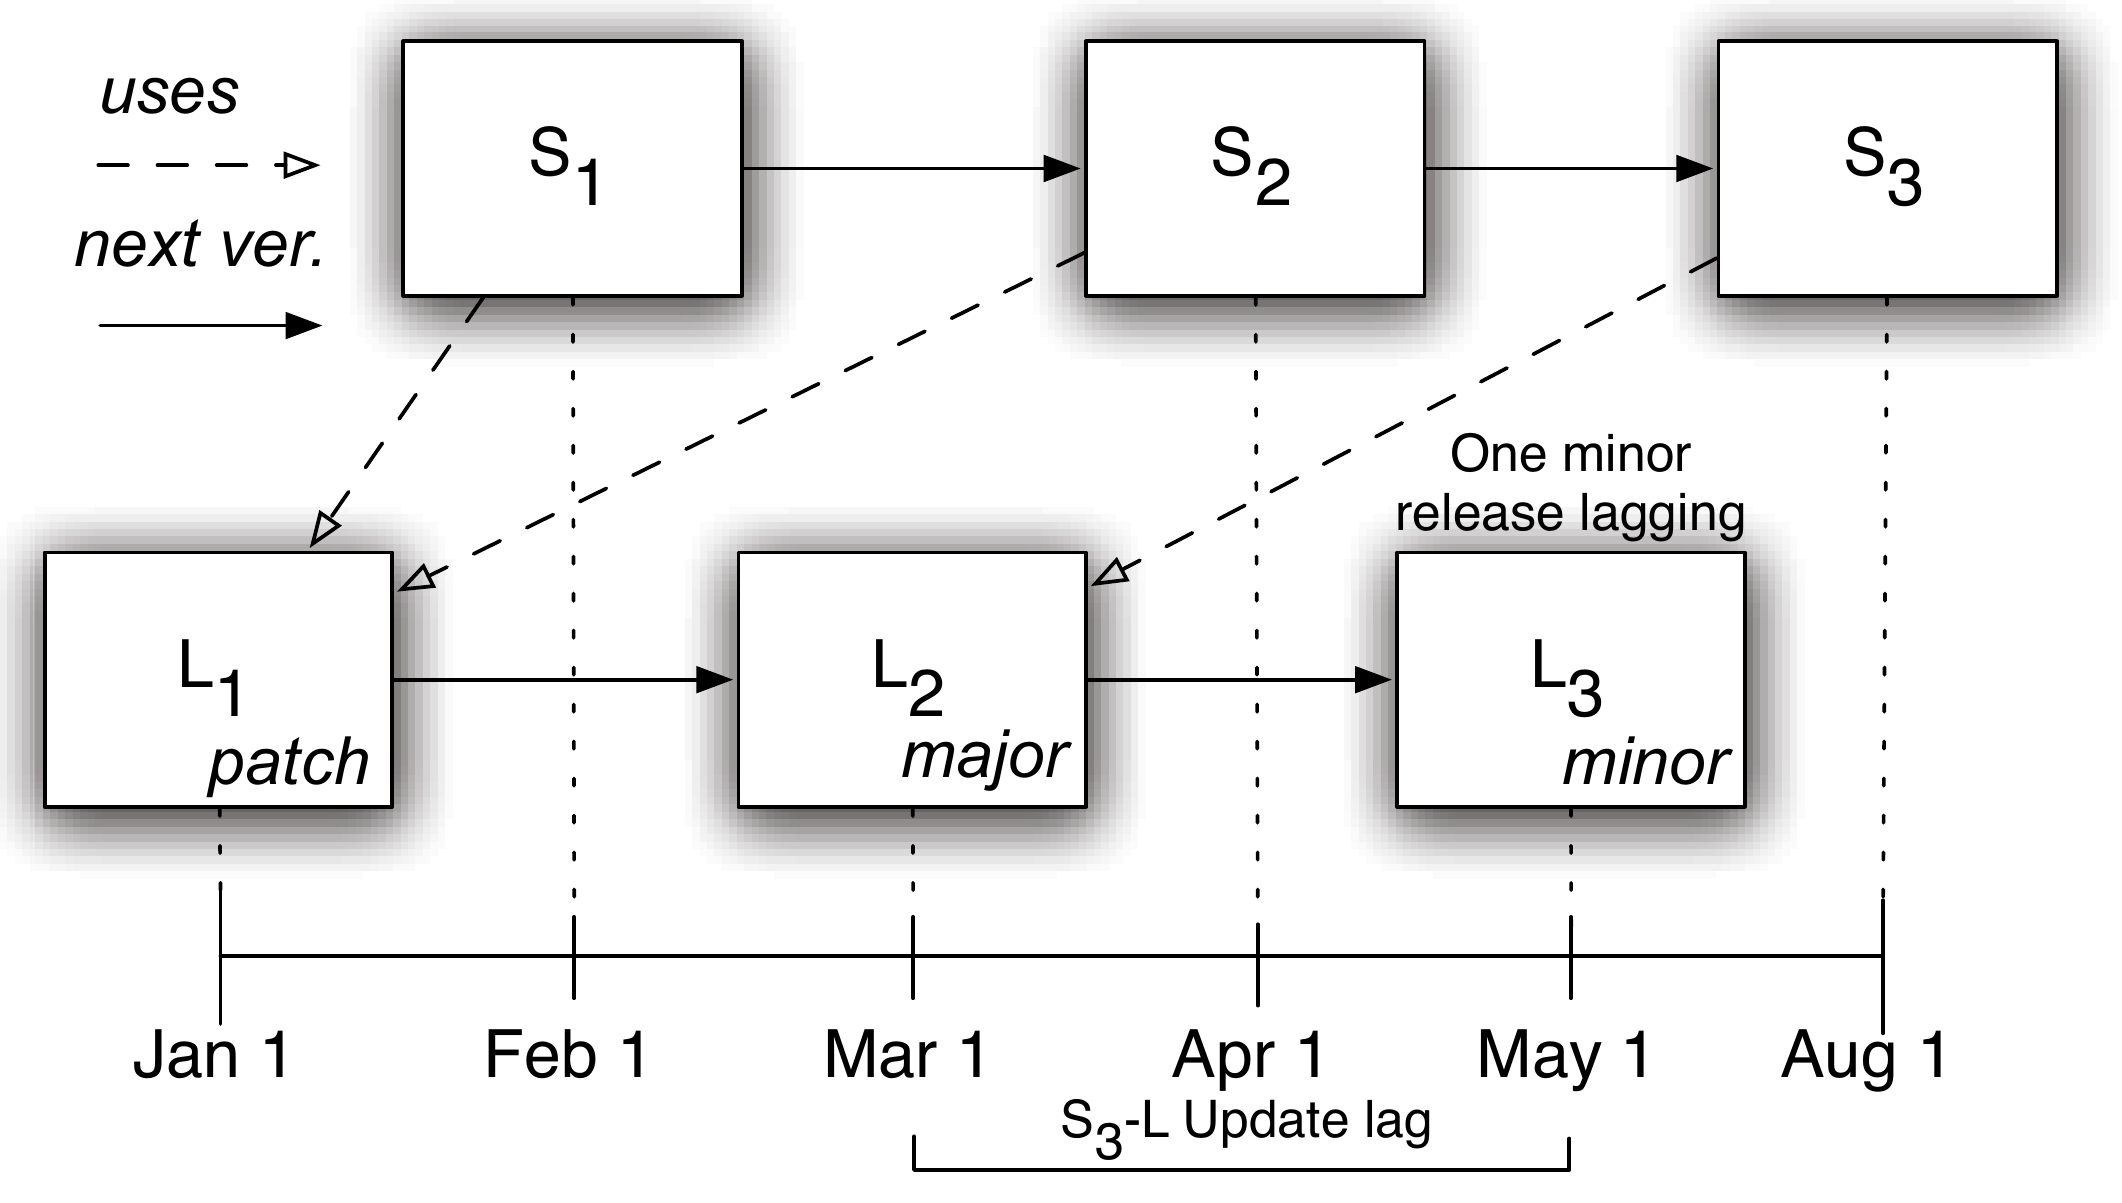
\includegraphics[width=\textwidth]{figure7}
\end{frame}
%%%%%%%%%%%%%%%%%%%%%%%%%%%%%%%%%%%%%%%%%%%%%%%%%%%%%%%%%%%%%%%%%%%%%%%%
\begin{frame}{RQ3-1:依存関係が伴う更新される数}

{\small
互換性がない更新に着目する理由は、依存関係の更新を困難に持たすから、
ここで依存関係の更新に関しても調べました。
}

ソフトウェアSの更新される際に、依存関係の記述にライブラリーLを伴って更新された数を調べた。

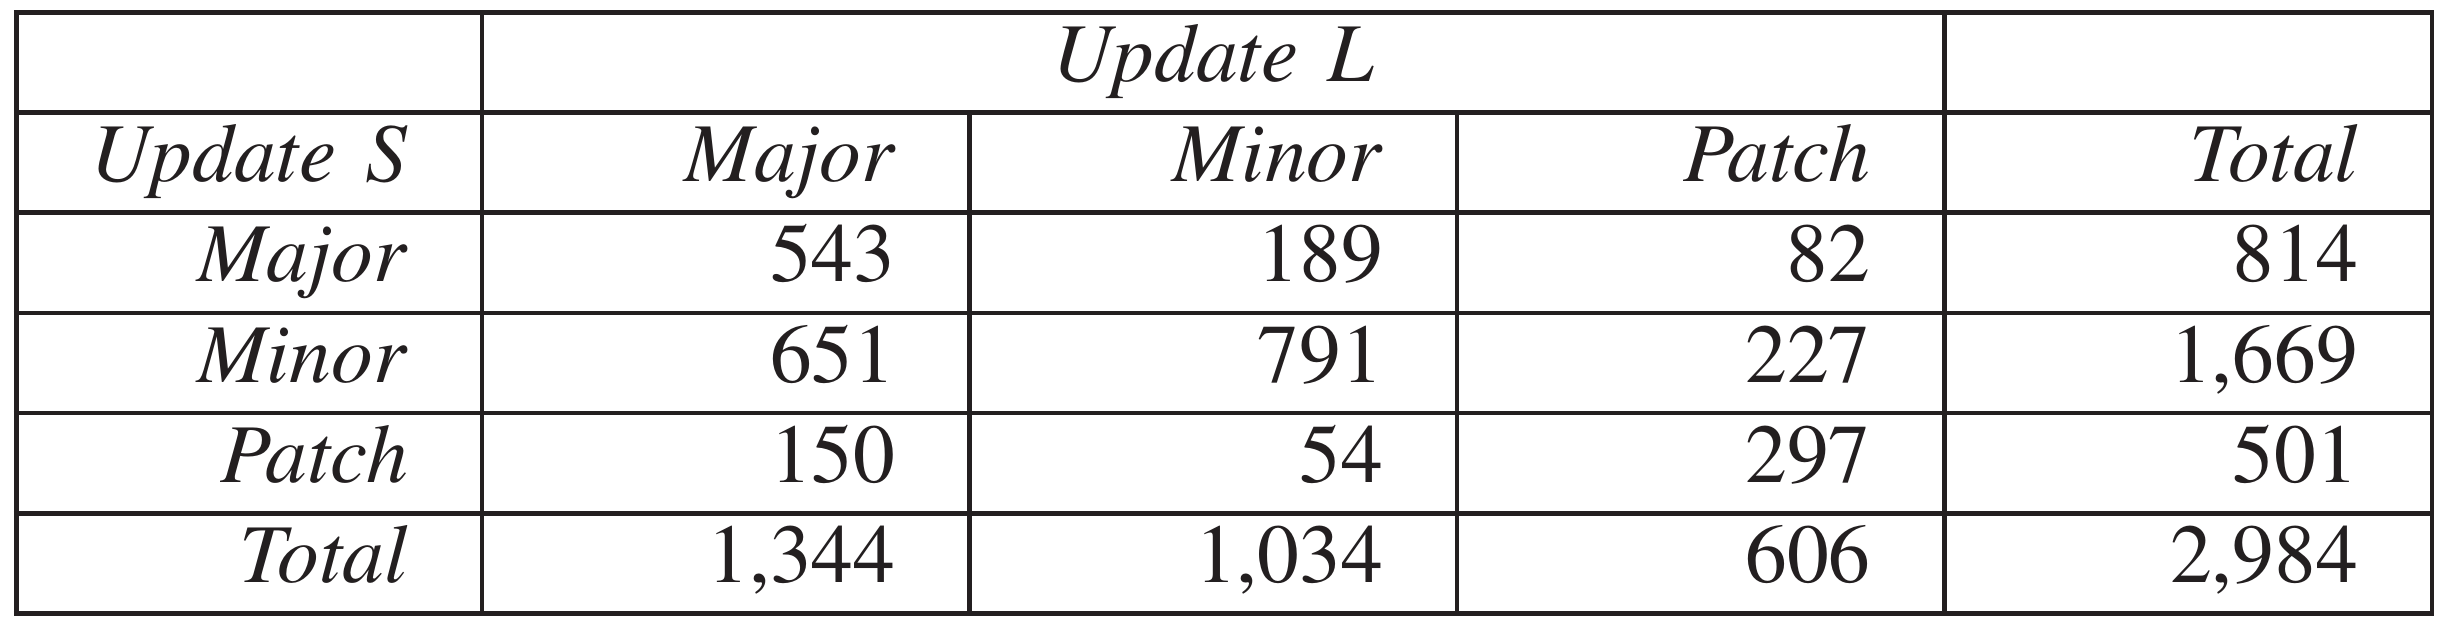
\includegraphics[width=\textwidth]{table6}

\end{frame}
%%%%%%%%%%%%%%%%%%%%%%%%%%%%%%%%%%%%%%%%%%%%%%%%%%%%%%%%%%%%%%%%%%%%%%%%
\begin{frame}{RQ3-2:依存関係が伴う更新の遅延}

{\small
更新の遅延: SがLを依存して、Lの最新版$L_n$がリリースされたが、
その後にリリースされたSの最新版は古い$L_o$に依存したまま場合、
一回の遅延と見なし、遅延の長さは$L_o$と$L_n$の間のリリースの数として定義。
}

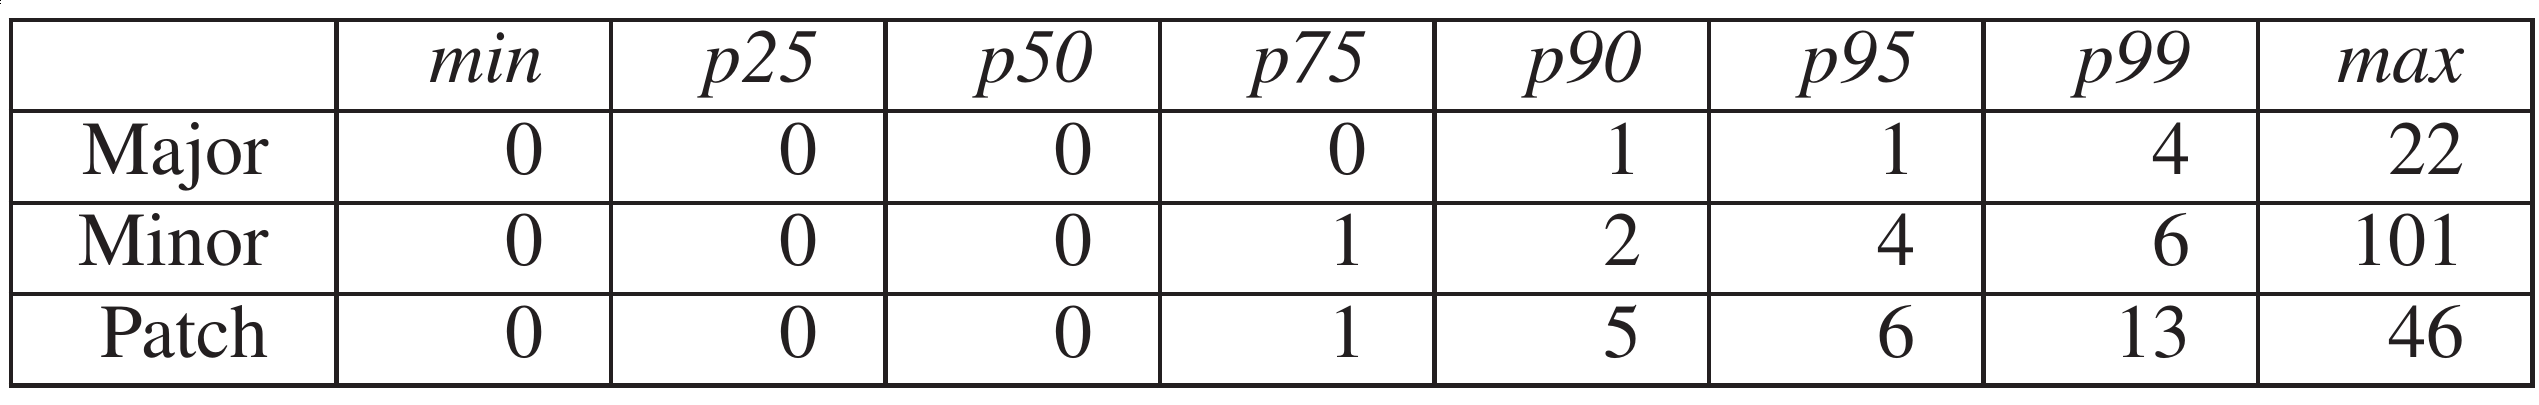
\includegraphics[width=\textwidth]{table8}

{\small
更新の遅延は互換性のない変更の数と
ソースコードに対する変更の激しさの関係を、
スピアマン相関係数で評価
}

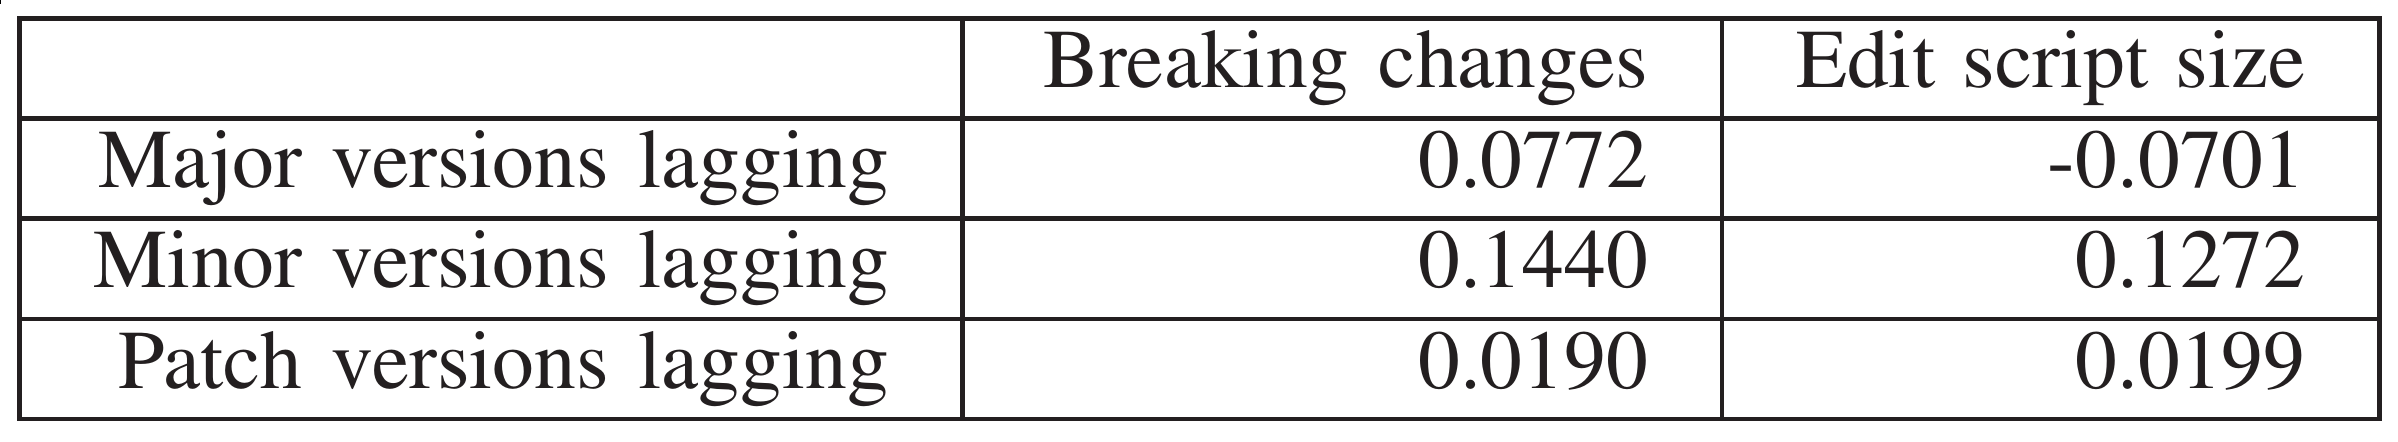
\includegraphics[width=\textwidth]{table9}

\end{frame}
%%%%%%%%%%%%%%%%%%%%%%%%%%%%%%%%%%%%%%%%%%%%%%%%%%%%%%%%%%%%%%%%%%%%%%%%
\begin{frame}{RQ3に対する回答}

{\Large
依存関係の更新は多くの場合に、ソフトウェアのMajorリリースにライブラリーのMajorリリースを更新される
}

\pause\vspace{1em}

{\Large
依存関係が更新するのに遅延が存在され、Patchリリースによく発生する
}

\pause\vspace{1em}

{\Large
更新の遅延は変化の激しさとの相関は弱いけど存在する
}

\end{frame}
%%%%%%%%%%%%%%%%%%%%%%%%%%%%%%%%%%%%%%%%%%%%%%%%%%%%%%%%%%%%%%%%%%%%%%%%
\subsection{RQ4:廃止予定タグが使われているか}
\begin{frame}[fragile]{廃止予定タグの正しい使い方}
\begin{columns}
\begin{column}{0.33\textwidth}
バージョン: 1.0
\begin{lstlisting}
class foo{

  public void 
  function(){
    //...
  };




}
\end{lstlisting}
\end{column}
\begin{column}{0.33\textwidth}
バージョン: 1.\textcolor{green!80!black}{1}
\begin{lstlisting}
 class foo{
+  @Deprecated
   public void 
   function(){
     //...
   };
+  public Object
+  functionEx(){
+    //...
+  };
 }
\end{lstlisting}
\end{column}
\begin{column}{0.33\textwidth}
バージョン: \textcolor{red}{2}.0
\begin{lstlisting}
 class foo{
-  @Deprecated
-  public void 
-  function(){
-    //...
-  };
   public Object 
   functionEx(){
     //...
   };
 }
\end{lstlisting}
\end{column}
\end{columns}
\end{frame}

%%%%%%%%%%%%%%%%%%%%%%%%%%%%%%%%%%%%%%%%%%%%%%%%%%%%%%%%%%%%%%%%%%%%%%%%

\begin{frame}{RQ4:廃止予定タグが使われているか}
22,205 プロジェクトの内、 1196 (5.4\%)は少なくとも一回メソッドに廃止予定のタグがつけられていた
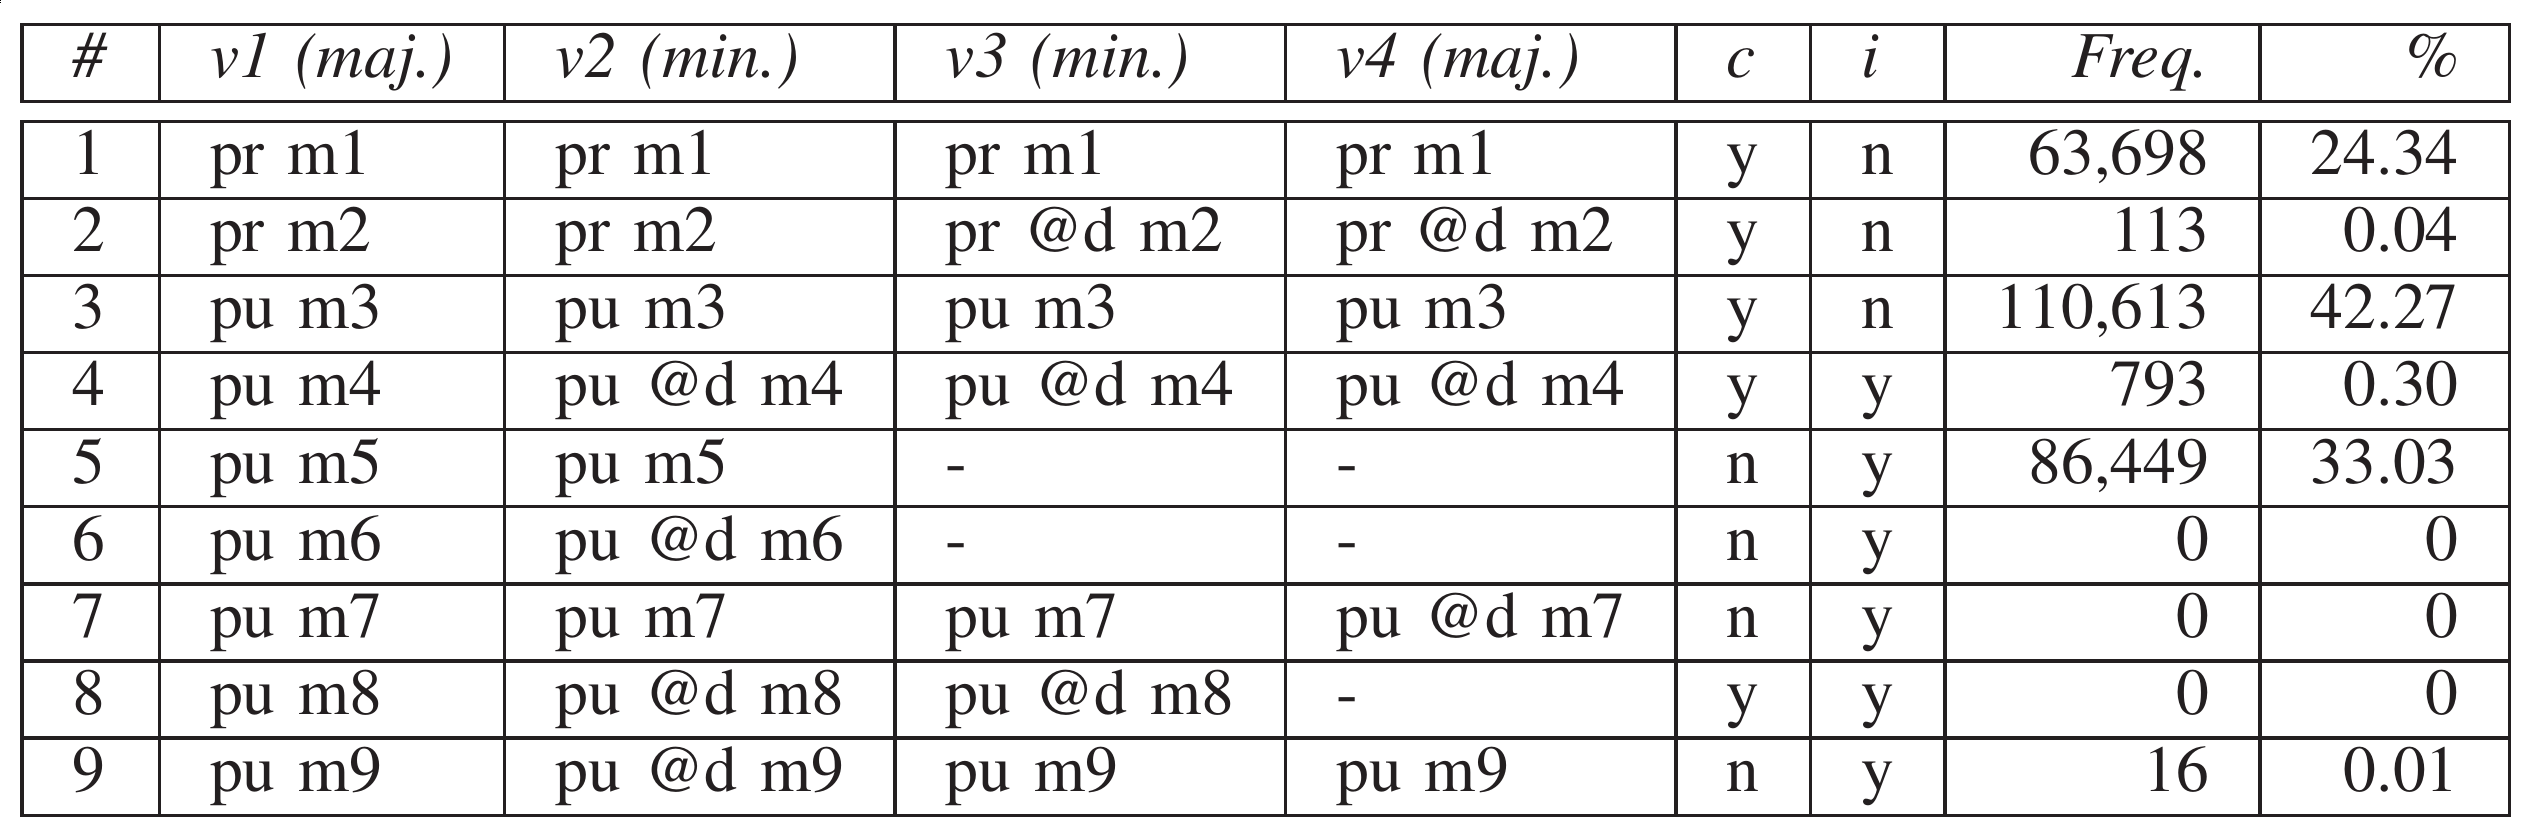
\includegraphics[width=\textwidth]{table10}

\begin{overlayarea}{\textwidth}{0.5\textheight}

\vspace{-1em}

\begin{itemize}
\item[1,2,3]<2> \texttt{private}や廃止と関係ないメソッドは対象外
\item[5,6,7]<3> 間違い使い方
\item[4,8]<4> 正しい使い方
\item[9]<5> 廃止予定がキャンセルした
\end{itemize}

\end{overlayarea}

\end{frame}

%%%%%%%%%%%%%%%%%%%%%%%%%%%%%%%%%%%%%%%%%%%%%%%%%%%%%%%%%%%%%%%%%%%%%%%%
\begin{frame}{RQ4に対する回答}

{\Large
プログラマーは廃止予定のタグを殆ど\textcolor{red}{使われていない}。
}

\pause\vspace{1em}

{\Huge
使われていても、\\
\textcolor{red}{正しく}使われていない。
}

\end{frame}

%%%%%%%%%%%%%%%%%%%%%%%%%%%%%%%%%%%%%%%%%%%%%%%%%%%%%%%%%%%%%%%%%%%%%%%%
\section{議論と妥当性への脅威}
\subsection{SemVer原則を守れない原因}
\begin{frame}{SemVer原則を守れない原因}{Low adherence explained}

{\small
Javaのモジュールシステムに可視性の設定はプログラマーの必要に満たせない。

「内部専用」のパケージは公開されてしまったことが多い。
}

\begin{tikzpicture}
\begin{umlpackage}[x=0,y=0]{software} 
\umlclass{UseImpl}{}{} 
\end{umlpackage} 
\begin{umlpackage}[x=4,y=0]{library}
\begin{umlpackage}{internal} 
\umlclass{PublicClassImpl}{}{} 
\end{umlpackage} 
\begin{umlpackage}[x=4,y=0]{external} 
\umlclass{PublicClass}{}{} 
\end{umlpackage} 
\end{umlpackage}
\end{tikzpicture}

実際の使い方と潜在的な使い方の違いもあります

\end{frame}
%%%%%%%%%%%%%%%%%%%%%%%%%%%%%%%%%%%%%%%%%%%%%%%%%%%%%%%%%%%%%%%%%%%%%%%%
\subsection{リリースの間隔と編集の規模}
\begin{frame}{リリースの間隔と編集の規模}
直感で考えると、MajorリリースはMinorリリースより時間がかかるはずなのに、
実際のデータから見る限り、\textcolor{red}{Minorリリースのほうが時間がかかります}。

\pause\vspace{1em}

推測: Majorリリースは意図的互換性を破るために作ることが多く、機能追加はその後にあるMinorリリースに行う。

\pause\vspace{1em}

ソースコードの編集の規模からもこの傾向が見えます:Minorリリースのほうが編集が多くされます。
\end{frame}
%%%%%%%%%%%%%%%%%%%%%%%%%%%%%%%%%%%%%%%%%%%%%%%%%%%%%%%%%%%%%%%%%%%%%%%%
\subsection{初期開発段階のリリース}
\begin{frame}{初期開発段階のリリース}
SemVer の説明によると「Major番号は0の場合(0.y.z)、互換性を守らないことは許されます」

\pause\vspace{1em}

今回の調査にこのルールを考慮していない。数だけを調べたら、Major番号は0のリリース数は
10.44\% (13,162 / 126,070) があります。

\end{frame}
%%%%%%%%%%%%%%%%%%%%%%%%%%%%%%%%%%%%%%%%%%%%%%%%%%%%%%%%%%%%%%%%%%%%%%%%
\subsection{妥当性への脅威}
\begin{frame}[shrink=10]{妥当性への脅威}
\begin{block}{内部的妥当性}
記録されたライブラリーのリリース日時が間違えた可能性がある。
\begin{itemize}
\item 2,321, 1.5\% のバイナリーファイルのリリース日時は 2005年11月5日になって、データから省いた
\item リリース日時の順位とバージョン番号によるソートした順位と一致しないことはある。
\end{itemize}

\end{block}

\begin{block}{外部的妥当性}
MavenにあるJavaで書かれたOSSだけ対象にした
\end{block}

\begin{block}{実験結果の再現性}
スーパーコンピューターで、100計算ノード、合計六ヶ月の計算時間を使って分析した
\end{block}
\end{frame}
%%%%%%%%%%%%%%%%%%%%%%%%%%%%%%%%%%%%%%%%%%%%%%%%%%%%%%%%%%%%%%%%%%%%%%%%
\section{結論}
\begin{frame}{結論}
この研究は22,000超えるMavenにあるOSSライブラリーを対象として、バージョン番号と
互換性の関係について、SemVerを基準として調査した。発見したことは:
\begin{itemize}
\item 互換性がない変更がよくある:$\frac{1}{3}$のリリース
\item majorバージョンであるかどうかと関わらず、互換性がない変更は同じぐらいに存在する
\item 互換性がない変更の存在は新しいライブラリーを使う遅延に影響は小さい
\item 廃止予定のタグはあまり使われていない、使った場合でも正しく使われていない
\end{itemize}
\end{frame}
%%%%%%%%%%%%%%%%%%%%%%%%%%%%%%%%%%%%%%%%%%%%%%%%%%%%%%%%%%%%%%%%%%%%%%%%

%%%%%%%%%%%%%%%%%%%%%%%%%%%%%%%%%%%%%%%%%%%%%%%%%%%%%%%%%%%%%%%%%%%%%%%%

\appendix
\backupbegin



\backupend
\end{document}
